\documentclass{article}
\usepackage{graphicx}
\usepackage{hyperref}
\usepackage{wrapfig}
\usepackage{float}
\usepackage{changepage} 
\usepackage[a4paper, total={6in, 10in}]{geometry}
\title{Intrusion Detection System Project Documentation}
\author{Adam Sin, Eliyahu Fridman}
\date{2024}

\begin{document}

\maketitle

\tableofcontents

\section{Introduction}
Our goal was to build an Intrusion Detection System (IDS) focusing on detecting packets suspicious of data exfiltration. We specifically examined the structure of packets to identify anomalies that could indicate malicious activities. The IDS was designed to sniff traffic on an interface, analyze each packet, and add the packet's general information to a list of sniffed packets, flagging those that failed certain tests along with the reason.

\newpage
\section{Project Structure}
\begin{figure}[H]
    \centering
    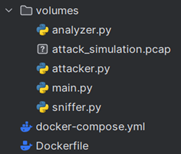
\includegraphics[width=0.4\textwidth]{structure.png}
\end{figure}

\subsection{Docker Setup}
The IDS is being run inside a Docker container for several reasons:
\begin{itemize}
    \item \textbf{Isolation}: By isolating the IDS inside a container, we ensure that only the intended traffic is analyzed. When running tests using TCP replay, we avoid interference from unrelated network packets.
    \item \textbf{Docker-Compose and Dockerfile}: The Docker Compose file set up the container, while the Dockerfile specified the necessary dependencies, such as \texttt{tkinter}, \texttt{pyshark}, and more.
\end{itemize}

\subsection{Attack Simulation (\texttt{attacker.py})}
This script’s only purpose is to create \texttt{attack\_simulation.pcap} which is used for the TCP replay testing each and every test the analyzer conducts on the packets.
The script creates a list with 132 packets, most of them meant to be suspicious of data exfiltration while a small amount are valid and their purpose will be explained later. The list is them used to create the pcap file using scapy’s wrpcap function.
All of the packets are outgoing, meaning they are sent from our company’s internal IPs to unknown external IPs. Because internal traffic shouldn’t cause data exfiltration unless we have a physical mole, external traffic has nothing to do with our company, and the assignment says to not test ingoing packets (from outside in).
\begin{figure}[H]
    \centering
    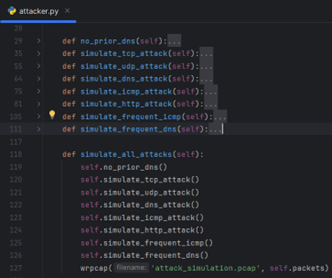
\includegraphics[width=0.4\textwidth]{attacker.png}
\end{figure} 

\newpage
\subsection{Sniffer (\texttt{sniffer.py})}
The Sniffer class, implemented in \texttt{sniffer.py}, is responsible for sniffing and storing network packets using \texttt{pyshark}'s \texttt{LiveCapture} function. The sniffer maintains a queue as a buffer, which the analyzer later uses to test the packets. It also includes a flag that determines whether to continue sniffing or stop.
\begin{figure}[H]
    \centering
    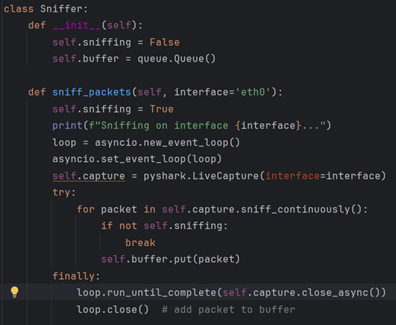
\includegraphics[width=0.4\textwidth]{sniffer.png}
\end{figure}

\subsection{Analyzer (\texttt{analyzer.py})}
The Analyzer class, implemented in \texttt{analyzer.py}, validates the captured packets by testing each packet to determine if it exhibits suspicious behavior. The \texttt{validate} function processes packets while the sniffer is active and there are packets to validate. \\
IsValid function is used to determine whether each packet is valid. 
It invokes several protocol-specific handlers to perform these checks:
\begin{figure}[H]
    \centering
    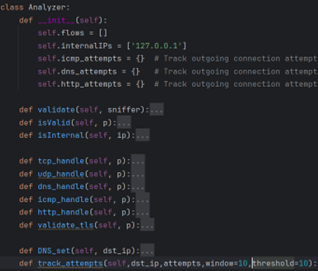
\includegraphics[width=0.4\textwidth]{analyzer.png}
\end{figure} 

\begin{itemize}
    \item \textbf{Is an outgoing packet?}: \\
    packets that are not outgoing don’t interest us:
    \begin{figure}[H]
        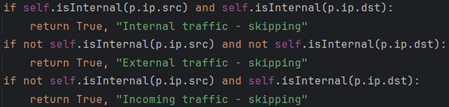
\includegraphics[width=0.4\textwidth]{test - isInternal.png}
    \end{figure}

    \newpage
    \item \textbf{TCP Handler}: \\
    Checks for usual tcp packet ports for secure traffic. Unusual ports may indicate tries to leak data unnoticed. More secure ports can and should be added. \\
    \begin{minipage}{\linewidth}
        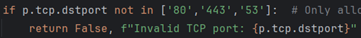
\includegraphics[width=0.4\textwidth]{test - tcp 1.png}
    \end{minipage}
    Tests for HTTPS packets on TCP protocol \\
    \begin{minipage}{\linewidth}
        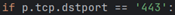
\includegraphics[width=0.4\textwidth]{test - tcp 2.png}
    \end{minipage}
    \begin{adjustwidth}{3em}{0em}
        A https packet must pass security tests, which is its purpose (tls tests are explained later) \\ 
        \begin{minipage}{\linewidth}
            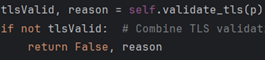
\includegraphics[width=0.4\textwidth]{test - tcp 2.1.png}\hspace{3em}
        \end{minipage}
        https packets sized more than 1460 bytes is unusual, we won’t allow sending so much data. \\
        \begin{minipage}{\linewidth}
            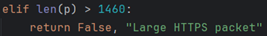
\includegraphics[width=0.4\textwidth]{test - tcp 2.2.png}\hspace{3em}
        \end{minipage}
    \end{adjustwidth}
    Unusually large TCP size might be a sign to leaked data in the payload. \\
    \begin{minipage}{\linewidth}
        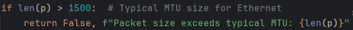
\includegraphics[width=0.4\textwidth]{test - tcp 3.png}
    \end{minipage}
    Both flags that represent both opening and closing a connection are very contrary and might be due to a try to use the server in an unusual way. \\ 
    \begin{minipage}{\linewidth}
        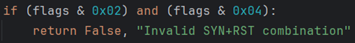
\includegraphics[width=0.4\textwidth]{test - tcp 4.png}
    \end{minipage}
    PSH flag means packets that should be processed by the receiver before any other given packets in the buffer. A packet too big of that importance might indicate a try to process and get the data fast. \\
    \begin{minipage}{\linewidth}
        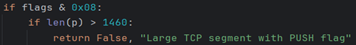
\includegraphics[width=0.4\textwidth]{test - tcp 5.png}
    \end{minipage}
    URG flag means packets with some important info that should be processed by the receiver before any other given packets in the buffer. A packet too big of that importance might indicate a try to process and get the data fast. \\ 
    \begin{minipage}{\linewidth}
        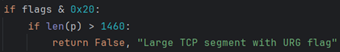
\includegraphics[width=0.4\textwidth]{test - tcp 6.png}
    \end{minipage}
% --------------------------------------------------------------------------------------- 
    \item \textbf{UDP Handler}: \\
    Checks for usual udp packet ports for secure traffic. Unusual ports may indicate tries to leak data unnoticed. More secure ports can and should be added. \\
    \begin{minipage}{\linewidth}
        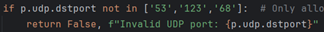
\includegraphics[width=0.4\textwidth]{test - udp 1.png}
    \end{minipage}
    NTP packets are for syncing servers and clients’ computers. This packet is usually sized 48 bytes so any other number of bytes is suspicious and should be checked for having different data. \\
    \begin{minipage}{\linewidth}
        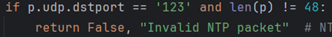
\includegraphics[width=0.4\textwidth]{test - udp 2.png}
    \end{minipage}
% --------------------------------------------------------------------------------------- 
    \item \textbf{DNS Handler}: \\
    If the packet is used as DNS \\
    \begin{minipage}{\linewidth}
        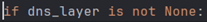
\includegraphics[width=0.4\textwidth]{test - dns 1.png}
    \end{minipage}
    \begin{adjustwidth}{3em}{0em}
        Any other port than 53, the usual port for DNS might be used for malicious causes. An example is trying to get a DNS response without being detected as a DNS request. \\
        \begin{minipage}{\linewidth}
            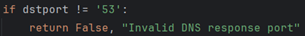
\includegraphics[width=0.4\textwidth]{test - dns 1.1.png}\hspace{3em}
        \end{minipage}
        DNS packets with a big payload indicates added data within getting leaked. \\
        \begin{minipage}{\linewidth}
            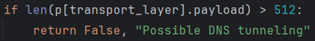
\includegraphics[width=0.4\textwidth]{test - dns 1.2.png}\hspace{3em}
        \end{minipage}
        \texttt{track\_attempts()} checks how many DNS responses were asked from the same IP and if too many   packets in a small window of time might be a try to leak data undetected using many small packets \\
        \begin{minipage}{\linewidth}
            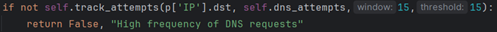
\includegraphics[width=0.4\textwidth]{test - dns 1.3.png}\hspace{3em}
        \end{minipage}
    \end{adjustwidth}

    if the packet is not a DNS packets with port 53 it may indicate a try to send data using a trusted port to not be detected. \\
    \begin{minipage}{\linewidth}
        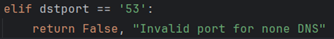
\includegraphics[width=0.4\textwidth]{test - dns 2.png}\hspace{3em}
    \end{minipage}
    For UDP packets that aren’t DNS we check that the payload doesn’t contain a DNS response. Secretly transmitted DNS responses should alert us. \\
    \begin{minipage}{\linewidth}
        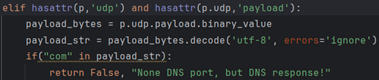
\includegraphics[width=0.4\textwidth]{test - dns 3.png}
    \end{minipage} 
    To get here means the packet has nothing to do with DNS. If so, \texttt{DNS\_set()} check that there was a valid DNS response before sending this packet. A case where a packet knew to be sent to our server without a DNS means someone knew in advance our information or were somehow under our radar. Both cases are suspicious and might be intended for data leaks. \\
    \begin{minipage}{\linewidth}
        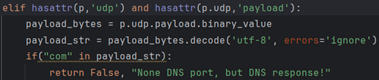
\includegraphics[width=0.4\textwidth]{test - dns 3.png}
    \end{minipage}
% ----------------------------------------------------------------------------------------
    \item \textbf{ICMP Handler}: \\
    ICMP packets with a big payload indicates added data within getting leaked. \\
    \begin{minipage}{\linewidth}
        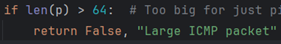
\includegraphics[width=0.4\textwidth]{test - icmp 1.png}
    \end{minipage}
    \texttt{track\_attempts()} checks how many ICMP responses were asked from the same IP and if too many   packets in a small window of time might be a try to leak data undetected using many small packets \\
    \begin{minipage}{\linewidth}
        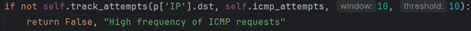
\includegraphics[width=0.4\textwidth]{test - icmp 2.png}
    \end{minipage}
% --------------------------------------------------------------------------------------- 
    \item \textbf{HTTP Handler}: \\
    HTTP packets with a big payload indicates added data within getting leaked. \\
    \begin{minipage}{\linewidth}
        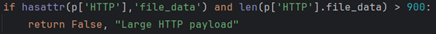
\includegraphics[width=0.4\textwidth]{test - http 1.png}
    \end{minipage}
    Host is a mandatory for HTTP 1.1 or higher in order to determine the specific site asking for response. Missing host in the header is unusual and may be to stay undetected. \\
    \begin{minipage}{\linewidth}
        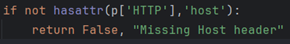
\includegraphics[width=0.4\textwidth]{test - http 2.png}
    \end{minipage}
    HTTP packets with a big header indicates added settings or data within getting leaked. \\
    \begin{minipage}{\linewidth}
        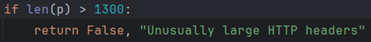
\includegraphics[width=0.4\textwidth]{test - http 3.png}
    \end{minipage}
    HTTP packets with these headers mean they contain sensitive information like passwords, permissions, etc. The server should be alerted if it wasn’t meant to be sent. \\
    \begin{minipage}{\linewidth}
        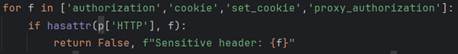
\includegraphics[width=0.4\textwidth]{test - http 4.png}
    \end{minipage}
    Requests that were sent using potentially malicious scripts may try extract data from the server. \\
    \begin{minipage}{\linewidth}
        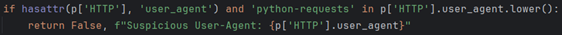
\includegraphics[width=0.4\textwidth]{test - http 5.png}
    \end{minipage}
    Allows sending data in chunks instead of all at once. Can be used to hide the amount of leaked data. \\
    \begin{minipage}{\linewidth}
        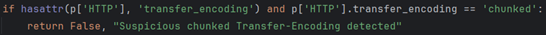
\includegraphics[width=0.4\textwidth]{test - http 6.png}
    \end{minipage}
    if the referrer that sent the request isn’t a trusted domain, we shouldn’t allow him to receive the response. \\
    \begin{minipage}{\linewidth}
        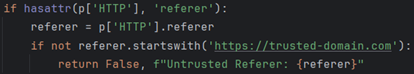
\includegraphics[width=0.4\textwidth]{test - http 7.png}
    \end{minipage}
    \texttt{track\_attempts()} checks how many HTTP responses were asked from the same IP and if too many   packets in a small window of time might be a try to leak data undetected using many small packets \\
    \begin{minipage}{\linewidth}
        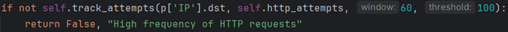
\includegraphics[width=0.4\textwidth]{test - http 8.png}
    \end{minipage}
% --------------------------------------------------------------------------------------- 
    \newpage
    \item \textbf{TLS Handler}: \\
    A HTTPS packet as to have a TLS layer by definition. \\
    \begin{minipage}{\linewidth}
        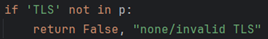
\includegraphics[width=0.4\textwidth]{test - tls 1.png}
    \end{minipage}
    Handshake types other than “Client Hello”, “Server Hello” in a TLS layer may be of a malicious intent. \\
    \begin{minipage}{\linewidth}
        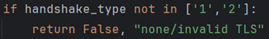
\includegraphics[width=0.4\textwidth]{test - tls 2.png}
    \end{minipage}
    A TLS without a SNI that supposed to contain information about the receiver may be due to security breaches or an untrusted connection. \\
    \begin{minipage}{\linewidth}
        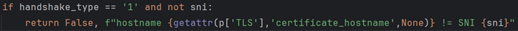
\includegraphics[width=0.4\textwidth]{test - tls 3.png}
    \end{minipage}
    if the TLS version is not secure enough might be to try and conduct malicious activity. \\
    \begin{minipage}{\linewidth}
        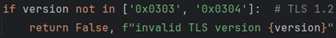
\includegraphics[width=0.4\textwidth]{test - tls 4.png}
    \end{minipage}
    if the cipher suite, which is the encryption algorithm aren’t secure enough, it may be so it will be easier to read leaked data. \\
    \begin{minipage}{\linewidth}
        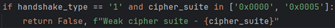
\includegraphics[width=0.4\textwidth]{test - tls 5.png}
    \end{minipage}
\end{itemize}


\subsection{Main Interface (\texttt{main.py})}
The main interface, implemented using \texttt{tkinter}, integrates the Sniffer, Analyzer, and Attacker components into a cohesive UI.
\begin{figure}[H]
    \centering
    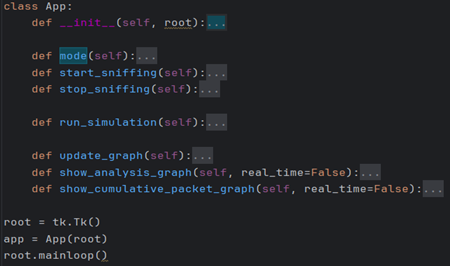
\includegraphics[width=0.4\textwidth]{main.png}
\end{figure}
To run the program:
\begin{itemize}
    \item Download Xlaunch from https://sourceforge.net/projects/vcxsrv/ 
    \item Run WSL
    \item Go to the docker-compose.yml and volumes directory.
    \item docker-compose build
    \item docker-compose up
    \item docker exec -it \texttt{protocols\_pyshark\_sniffer\_1} bash
    \item cd volumes
    \item python3 main.py
\end{itemize}

\newpage
Running the program provides the following functionality:
\begin{itemize}
    \item \textbf{Start Sniffing}: will run the sniffer across the interface inside the docker. Another click will stop.
    \item \textbf{Run Simulation}: will use TCP replay to simulate the pcap across the interface so the sniffer could sniff the packets and have the analyzer test them.
    \begin{figure}[H]
        \centering
        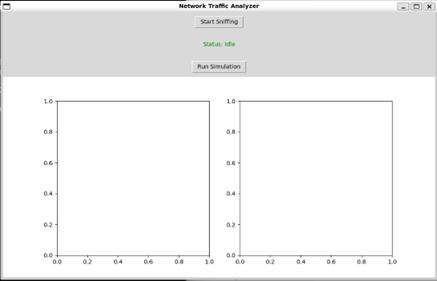
\includegraphics[width=0.4\textwidth]{gui 1.png}
    \end{figure}
    \item \textbf{Statistics Display}: Graphically presents analysis results using Matplotlib, showing cumulative packet counts and protocol breakdowns.
    \begin{figure}[H]
        \centering
        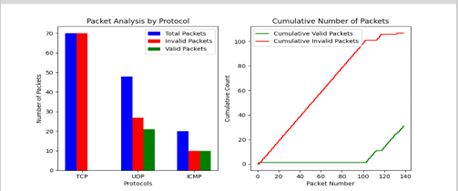
\includegraphics[width=0.4\textwidth]{gui 2.png}
    \end{figure}
    \textbf{Packets Analysis by protocol}: \\
    for each protocol TCP,UDP,ICMP we count: \\
    Blue - the number of packets sniffed \\
    green - the number of valid packets sniffed \\
    red - the number of packets that are suspicious of data exfiltration that were sniffed

    \textbf{Cumulative Number of Packets}: \\
    We want to see the cumulative number of  valid/invalid packets over time: \\
    Red – the cumulative number of packets that are suspicious of data exfiltration \\
    Green - the cumulative number of valid packets
\end{itemize}

\end{document}
